\documentclass[a4paper,article,14pt]{extarticle}

\usepackage{spbudiploma}
\usepackage{amsmath}
\usepackage{mathtools}
\usepackage[pdftex]{graphicx}
\graphicspath{{../pictures/}}
\usepackage{listings}
\usepackage{xcolor}
\usepackage{amsfonts}
\usepackage{amsmath}
\usepackage{cases}

\usepackage{enumitem}
\definecolor{codegreen}{rgb}{0,0.6,0}
\definecolor{codegray}{rgb}{0.5,0.5,0.5}
\definecolor{codepurple}{rgb}{0.58,0,0.82}
\definecolor{backcolour}{rgb}{0.95,0.95,0.92}

\lstdefinestyle{mystyle}{
	backgroundcolor=\color{backcolour},   
	commentstyle=\color{codegreen},
	keywordstyle=\color{codegreen},
	numberstyle=\tiny\color{codegray},
	stringstyle=\color{codepurple},
	basicstyle=\ttfamily\footnotesize,
	breakatwhitespace=false,         
	breaklines=true,                 
	captionpos=b,                    
	keepspaces=false,                 
	numbers=left,                    
	numbersep=5pt,                  
	showspaces=false,                
	showstringspaces=false,
	showtabs=false,                  
	tabsize=2
}

\lstset{style=mystyle}

\begin{document}
	\begin{titlepage}
		\begin{center}
			FEDERAL STATE AUTONOMOUS EDUCATIONAL INSTITUTION
			
			OF HIGHER EDUCATION
			
			ITMO UNIVERSITY
			\vspace{3cm}
			
			\large\textbf{Report}
			
			\large on the practical task No. 5
			
			\large \flqq Algorithms on graphs. \\ Introduction to graphs and basic algorithms on graphs\frqq
			\vspace{5cm}
			

			\begin{flushright}
				{Performed by:} \\
				Putnikov Semyon \\ 
				J4132c \\
			\end{flushright}
			
			
			\begin{flushright}
				{Accepted by:} \\
				Dr Petr Chunaev \\ 
			\end{flushright}
			\vfill
			
			{St. Petersburg}
			\par{\number\year}
		\end{center}
	\end{titlepage}

	\newpage
	
	\section{Goal}
	The use of different representations of graphs and basic algorithms on graphs (Depth-first search and Breadth-first search).
	
	\section{Formulation of the problem}
	\begin{enumerate}[label=\Roman*]
		\item Generate a random adjacency matrix for a simple undirected unweighted graph with 100 vertices and 200 edges (note that the matrix should be symmetric and contain only 0s and 1s as elements). Transfer the matrix into an adjacency list. Visualize the graph and print several rows of the adjacency matrix and the adjacency list. Which purposes is each representation more convenient for?
		\item Use Depth-first search to find connected components of the graph and Breadth-first search to find a shortest path between two random vertices. Analyse the results obtained.
		\item Describe the data structures and design techniques used within the algorithms.
	\end{enumerate}
	
	\section{Brief theoretical part}
	\subsection{Depth-first search (DFS)}
	Depth-first search (DFS) is an algorithm for traversing or searching a graph. The algorithm starts at a chosen root vertex and explores as far as possible along each branch before backtracking. Applied for: searching connected components, searching loops in a graph, testing bipartiteness, topological sorting, etc.
	
	The time complexity of DFS is $O(|V|+|E|)$.
	
	A connected component of a graph is a subgraph in which any two vertices are connected by paths, and which is not connected to any vertex in the rest graph.
	
	\subsection{Breadth-first search (BFS)}
	Breadth-first search (BFS) is an algorithm for traversing or searching a graph. The algorithm starts at a chosen root vertex and explores all of the neighbour vertices at the present depth prior to moving on to the vertices at the next depth level. It uses an opposite strategy to DFS, which instead explores the vertex branch as far as possible before being forced to backtrack and expand other vertices. 
	
	Applied for: searching shortest path.
	
	The time complexity of BFS is $O(|V|+|E|)$.
	
	
	
	
	\section{Results}
	%Present the results of solving the assigned problems, including graphs and tables, as well as a brief discussion of the results obtained (at most 4 pages)
	
	In theory for sparse graph adjacency matrix fit into more memory than adjacency list, but also exist sparse data structures which erase this drawback. The main drawback of this adjancy list is that there is no quick way to check existence of edge (u, v).

	\begin{figure}[h!]
		\centering
		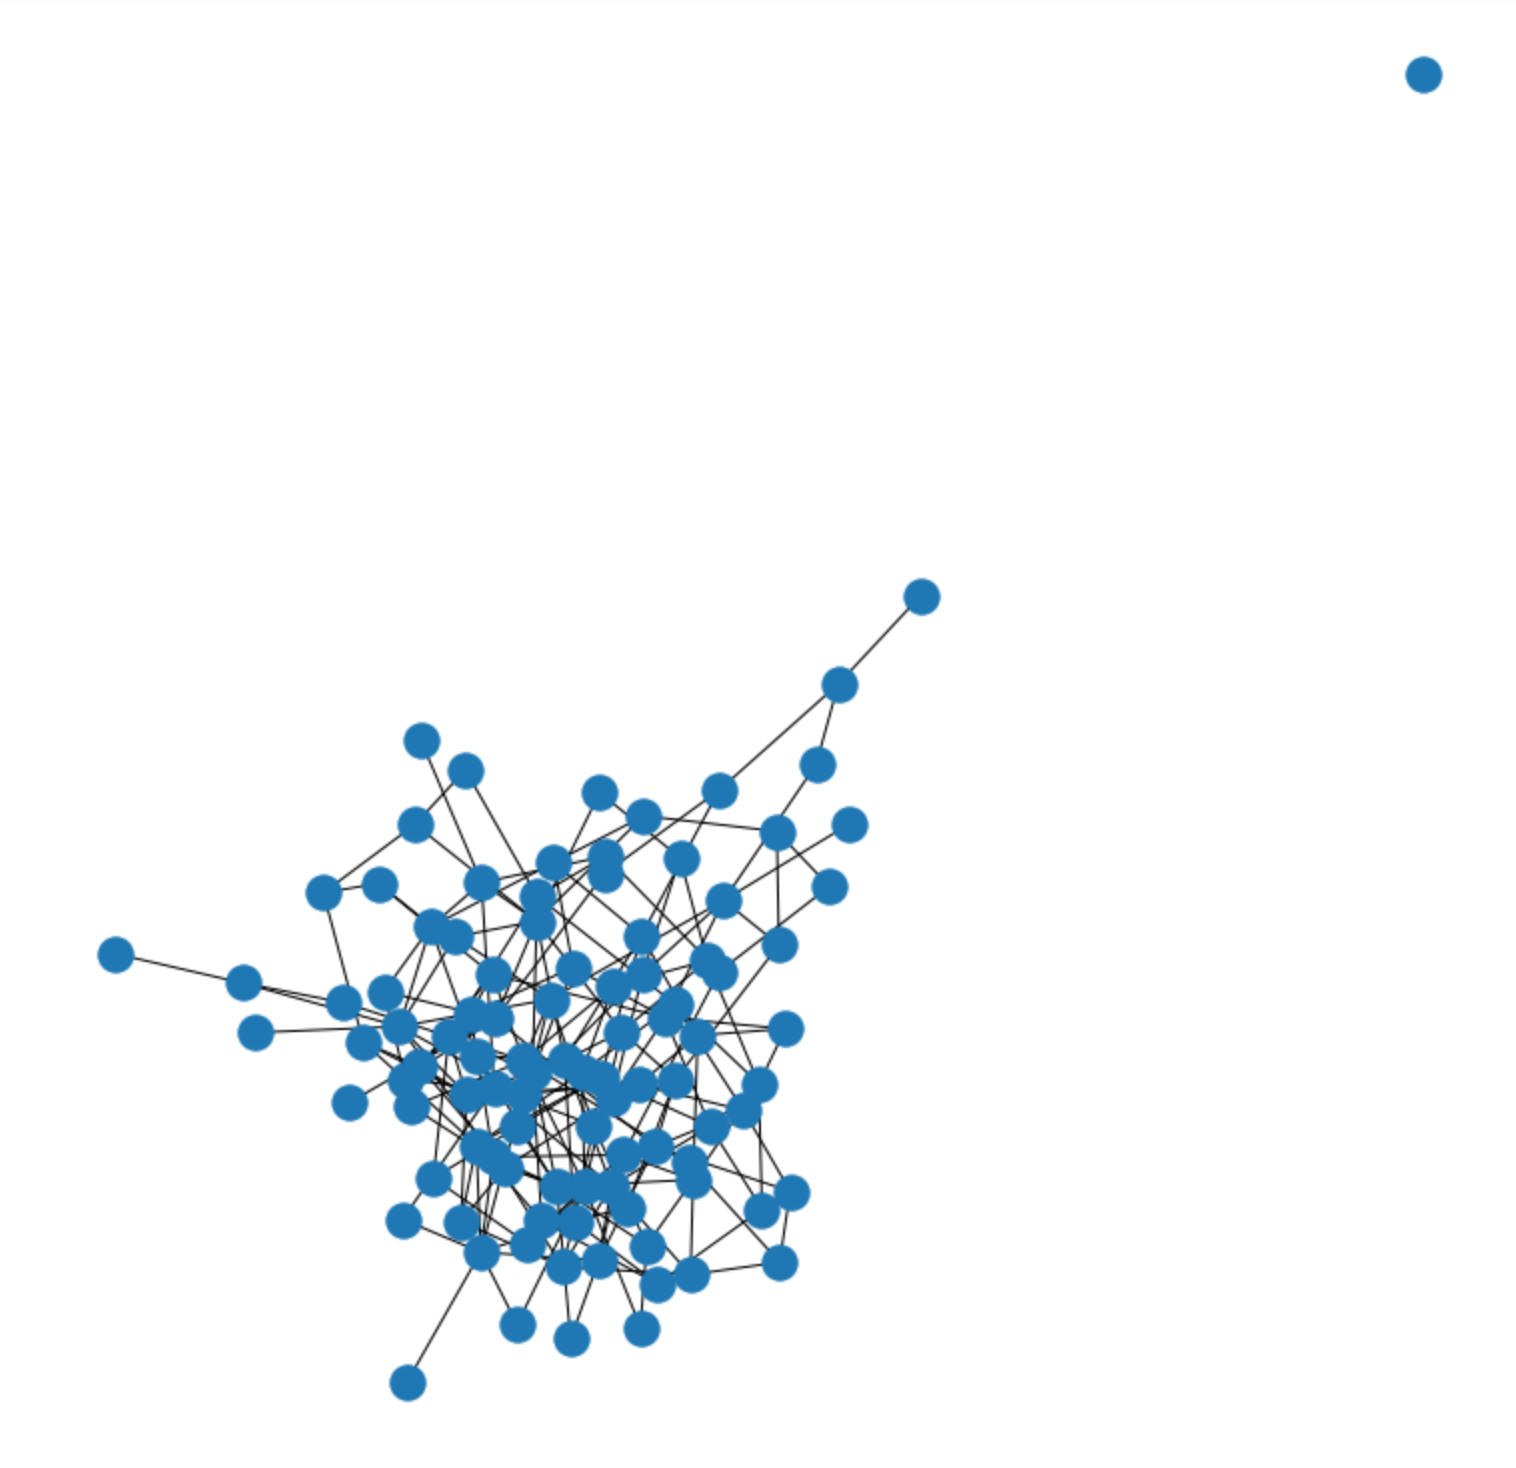
\includegraphics[scale=0.7]{graph.png}
		\caption{Graph visualization.}
		\label{graph}
	\end{figure}


	\begin{figure}[h!]
		\centering
		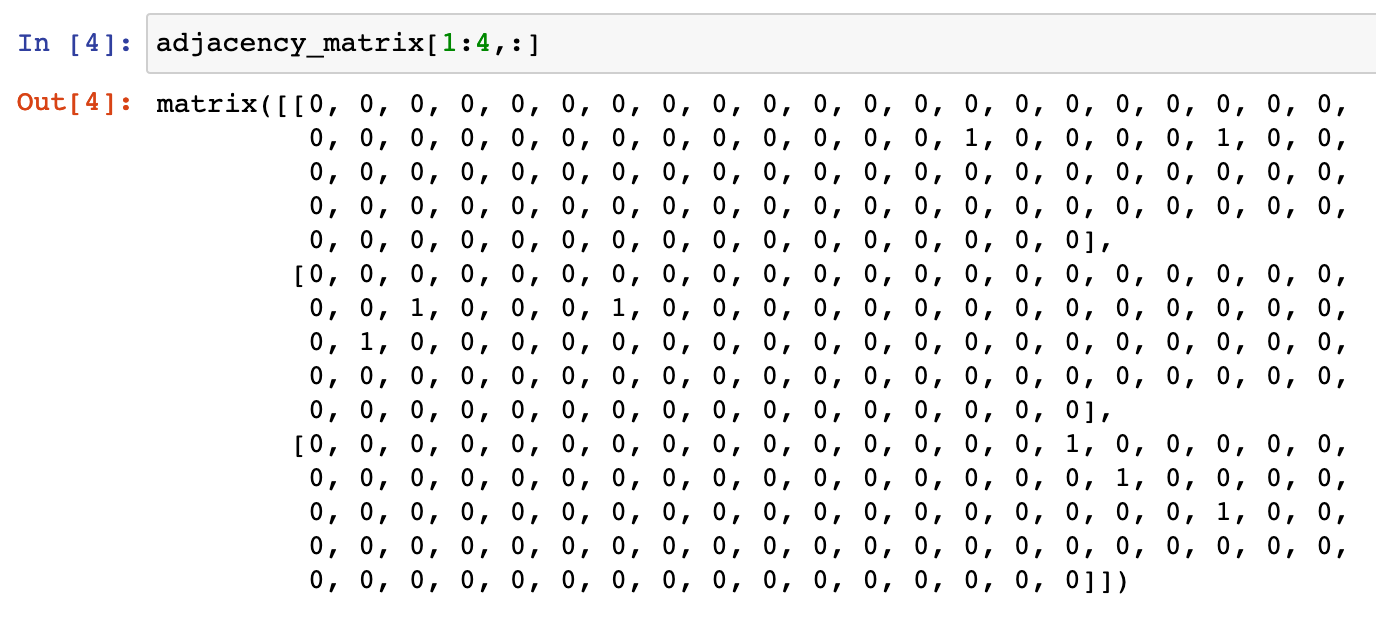
\includegraphics[scale=0.35]{adjacency_matrix.png}
		\caption{Adjacency matrix.}
		\label{matrix}
	\end{figure} 

	\begin{figure}[h!]
		\centering
		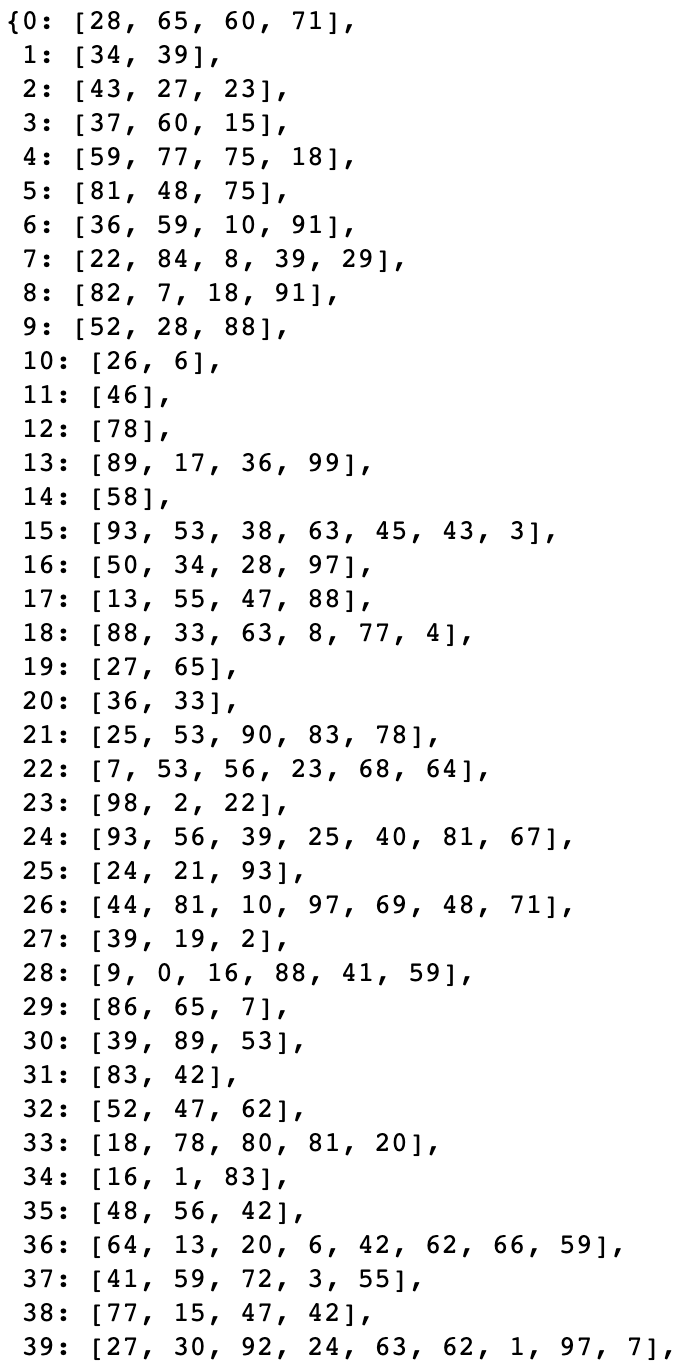
\includegraphics[scale=0.35]{adjacency_list.png}
		\caption{Adjacency list.}
		\label{list}
	\end{figure} 

	As we can see on graphs visualization which have 100 nodes and 200 edges visualization of graphs not worthless only for very small graphs. 
	
	\begin{figure}[h!]
		\centering
		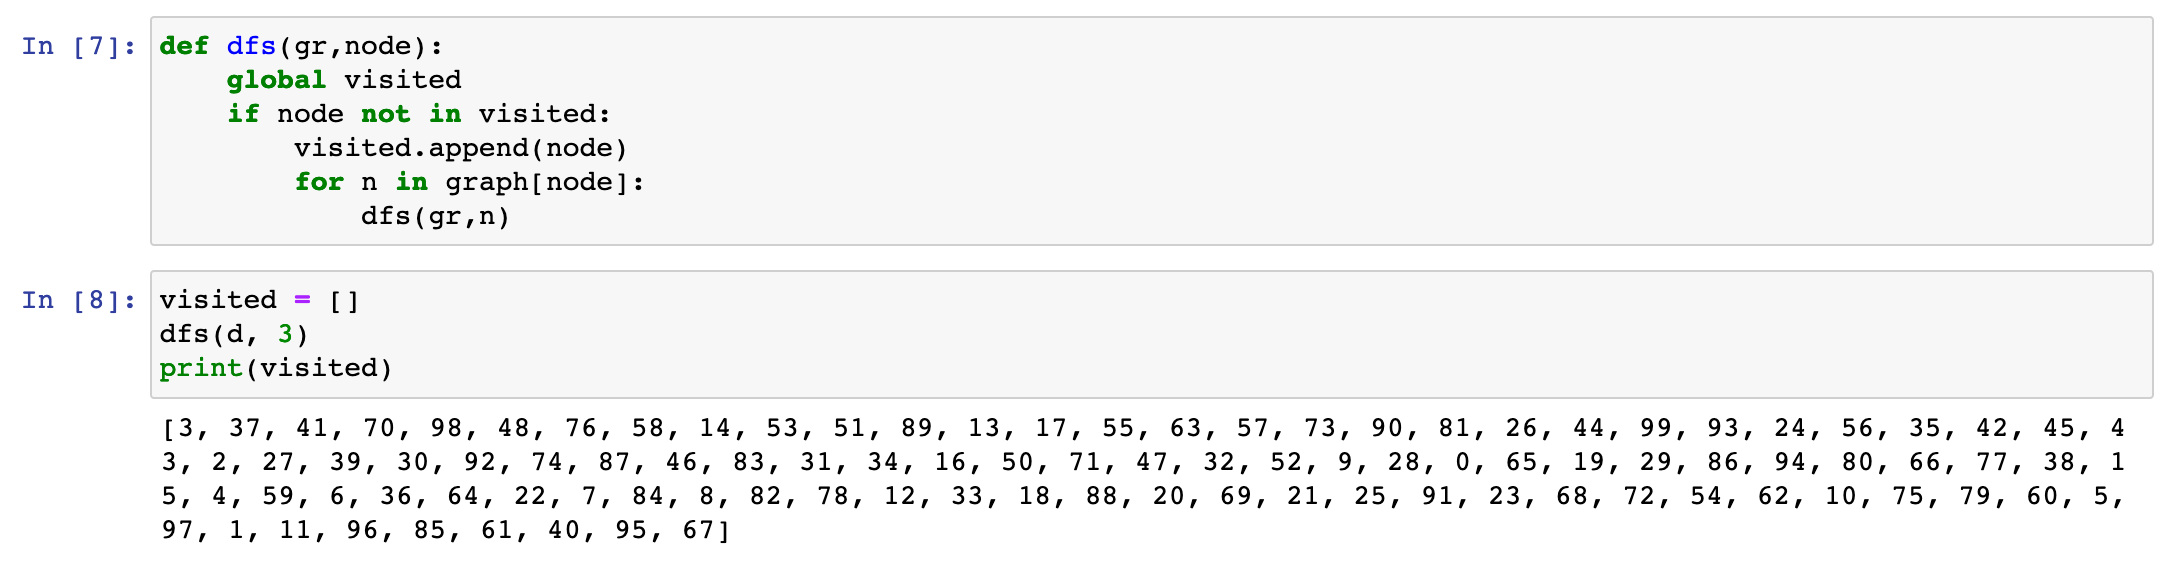
\includegraphics[scale=0.35]{dfs.png}
		\caption{Results of dfs calculations.}
		\label{dfs}
	\end{figure} 
	
	\begin{figure}[h]
		\centering
		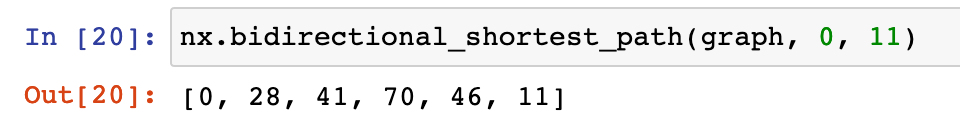
\includegraphics[scale=0.35]{bfs.png}
		\caption{Results of bfs calculations.}
		\label{bfs}
	\end{figure} 
	
	Using DFS we can obtain number of components in graph and connected problems. Using BFS is one of ways which we can get shortest path between 2 nodes.
	
	I used dictionaries and lists for programming visualization of above algorithms. Also I used recursive technique.

	
\end{document}